% !TEX TS-program = pdflatex
% !TEX encoding = UTF-8 Unicode

\documentclass[UTF8, a4paper, 12pt]{report}
	\title{模式识别作业\\——CNN分类器}
	\author{汪皓 202020116491}
	\date{2020/12/29}

\usepackage{ctex}
\usepackage{amsmath}
\usepackage{amssymb}
\usepackage{titlesec} % set Chapter1 to chinese 第一章
\usepackage{zhnumber}
\titleformat{\chapter}{\raggedright\Huge\bfseries}{第\,\zhnum{chapter}\,章}{1em}{}
 \usepackage{indentfirst} % 首行缩进
\usepackage{enumitem} % 序号
\usepackage{graphicx} % 插图
\makeatletter
\newcommand*\bigcdot{\mathpalette\bigcdot@{.5}}
\newcommand*\bigcdot@[2]{\mathbin{\vcenter{\hbox{\scalebox{#2}{$\m@th#1\bullet$}}}}}
\makeatother

\usepackage{subfigure}

\usepackage[noend]{algpseudocode}
\usepackage{algorithmicx,algorithm}

\usepackage{bm}
\usepackage{float}
\usepackage{tikz} % 流程图
\usetikzlibrary{shapes, arrows}
\tikzstyle{startstop} = [rectangle,rounded corners, minimum width=3cm,minimum height=1cm,text centered, draw=black,fill=red!30]
\tikzstyle{io} = [trapezium, trapezium left angle = 70,trapezium right angle=110,minimum width=3cm,minimum height=1cm,text centered,draw=black,fill=blue!30]
\tikzstyle{process} = [rectangle,minimum width=3cm,minimum height=1cm,text centered,text width =3cm,draw=black,fill=orange!30]
\tikzstyle{decision} = [diamond,minimum width=3cm,minimum height=1cm,text centered,draw=black,fill=green!30]
\tikzstyle{arrow} = [thick,->,>=stealth]

\usepackage{dirtree} % 目录树绘制

\usepackage{fancyhdr} % use this package to set page
\pagestyle{fancy}
\lhead{}
\rhead{}
\chead{\leftmark} % set all the headings in the center of the page
\lfoot{}
\rfoot{}
\cfoot{\thepage}
\renewcommand{\headrulewidth}{0pt} % set off the line over the heading

% \usepackage[left=2.50cm, right=2.50cm, top=2.50cm, bottom=2.50cm]{geometry} % page distance
\usepackage[top=2.50cm, bottom=2.50cm]{geometry}


\begin{document}
% \CJKindent
\maketitle % generate the document title
\thispagestyle{empty} % this page with no page number
\clearpage % create a new page

\pagestyle{plain} % set the content with no heading, but a page number
\setcounter{page}{1} % set the content page as Page I
\pagenumbering{Roman} % set the I(Roman)
\tableofcontents % generate the content
\clearpage

\pagestyle{fancy} % the main body use fancy
\setcounter{page}{1} % set the main body page as Page 1
\pagenumbering{arabic} % set the 1(arabic)

\chapter{实验目的}
	\section{实验要求}
		设计并实现一个基于最小错误率贝叶斯方法的手写数字识别系统,并实现以下功能:
		\begin{enumerate}[itemindent=1em]
			\renewcommand{\labelenumi}{\theenumi)}
			\item 搭建平台;(确定编程环境,构建实验平台框架)
			\item 特征描述;
			\item 建立基于最小错误率的贝叶斯决策分类器;
			\item 实现手写数字识别
		\end{enumerate}

	\section{实验思路}
		整个实验要求搭建一个手写数字识别系统,故总体来说需要实现三个模块:用户交互界面(GUI)模块、特征提取与处理模块、监督学习算法训练与识别模块。以下几章将从如上所述几个方面分别展开。总体实验框架如图1.1所示。

	\section{实验意义}
		通过设计手写数字识别系统,深入理解模式识别的总体框架、特征提取和各种算法,对模式识别这一方向有更深入的理解,对自动化与人工智能整体方向有更深入的理解。在工程实现的过程中,加强代码能力和解决问题的能力。
		\begin{figure}
			\centering
			\begin{tikzpicture}[node distance=2cm]
				\node (start) [startstop] {Start};
				\node(ui) [startstop, below of=start]{GUI};
				\node (write) [io, below of=ui] {手写数字};
				\node (selection) [decision, below of=write, yshift=-0.75cm] {训练识别};
				\node (save) [process, right of=selection, xshift=3cm] {保存图片};
				\node (recog) [process, below of=selection, yshift=-0.75cm] {识别};
				\node (train) [process, right of=recog, xshift=3cm] {算法训练};
				\node (end) [startstop, below of=recog] {End};
	     
				%连接具体形状
				\draw [arrow](start) -- (ui);
				\draw [arrow](ui) -- (write);
				\draw [arrow](write) -- (selection);
				\draw [arrow](selection) -- node[anchor=south]{save}(save);
				\draw [arrow](save) --(train);
				\draw [arrow](save) |- (ui);
				\draw [arrow](selection) -- node[anchor=east]{recognize}(recog);
				\draw [arrow](train) -- (recog);
				\draw [arrow](recog) -- (end);

			\end{tikzpicture}
			\caption{总体实验框架(流程图)}
			\label{fig:1.1}
		\end{figure}


\clearpage

\chapter{实验平台}
	\section{编程环境}
		鉴于个人对python语言的了解较其他语言丰富,故在实现过程中,采用python作为主要使用的编程语言,在pycharm平台上进行GUI设计。设计过程中所使用的语言、编程环境及主要依赖库的详细信息如表2.1:
		\begin{table}[!h]
		\centering
		\caption{实验环境信息}  
		\begin{tabular*}{13cm}{lll}  
		\hline  
		名称 & 版本  & 描述 \\  
		\hline  
		\hline
		python  & 3.7.9 & 编程语言 \\  
		pycharm  & community-2020.2 & 集成开发环境(编程、调试、运行) \\  
		PyQt5 & 5.15.1 & GUI设计\\
		PyTorch & 1.6.0+cpu & 数学运算及算法实现\\  
		Torchvision & 0.7.0+cpu & 数据特征处理\\
		PIL & 7.2.0 & 图片读取和特征处理\\
		\hline  
		\end{tabular*}  
		\end{table}  

	\section{平台搭建}
		\subsection{PyQt5简介}
			PyQt5是基于Digia公司强大的图形程式框架Qt5的python接口,由一组python模块构成。PyQt5本身拥有超过620个类和6000函数及方法。在可以运行于多个平台,包括:Unix, Windows, and Mac OS。\\
			PyQt5有自己的图形界面,也有封装在python里的内嵌库,在这里,为了与我们的算法融合,我们选用PyQt5内嵌于python的库。PyQt5分为很多模块,主要模块有:
			\begin{enumerate}[itemindent=1em]
				\renewcommand{\labelenumi}{•}
				\item QtCore 包含了核心的非GUI的功能。主要和时间、文件与文件夹、各种数据、流、URLs、mime类文件、进程与线程一起使用。
				\item QtGui 包含了窗口系统、事件处理、2D图像、基本绘画、字体和文字类。
				\item QtWidgets 包含了大多数GUI设计需要的工具、插件和窗体,是在Qt中创建用户界面的主要元素。
				\item QtMultimedia
			\end{enumerate}

		\subsection{画板实现}
			画板是用户交互的主要界面,其作用是实现手写数字的输入和读取,涉及到的插件和工具有:QWidget、QPixemap、QPainter、QPoint、QPen、QMouse等,其作用如表2.2所示。
			\begin{table}[!h]
			\centering
			\caption{画板设计所涉及相关插件及工具介绍}  
			\begin{tabular*}{13cm}{lll}  
			\hline  
			名称 & 描述 \\  
			\hline  
			\hline
			QWidget  & 作为画板设计的窗口 \\  
			QPixemap  & 用于图片的读写与显示 \\  
			QPainter & 作画工具(画笔的外壳)\\
			QPoint & 鼠标位置与画板位置获取\\  
			QPen & 画笔(内部属性)\\
			QMouse & 获取鼠标动态\\
			\hline  
			\end{tabular*}  
			\end{table}  
		
			如图2.1所示,使用画布可以实现手写板功能。用户通过鼠标在画板上写数字,画板记录并保存手写数字,用于算法训练和识别。
			\begin{figure}[H]
			\centering
			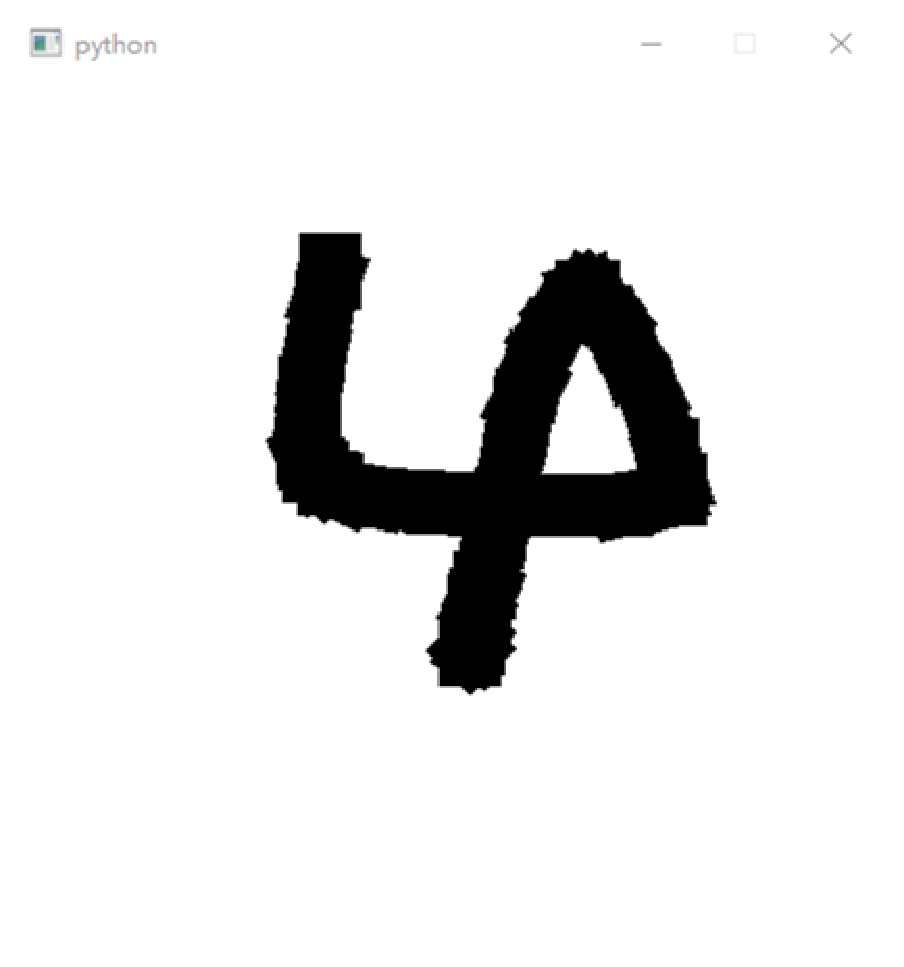
\includegraphics[scale=0.5]{./img/PaintBoard.eps}
			\caption{画布界面展示}
			\label{fig:2.1}
			\end{figure}

		\subsection{GUI实现}
			将前述画布作为一个插件布局到一个较大QWidget窗口之中,利用QLabel、QTextEdit、QLineEdit、QCheckBox、QIcon等等实现整体GUI布局,如图2.2所示。再在该窗口外面套一层QMainWindow制成的窗体,形成最终的应用窗口。
			\begin{figure}[H]
			\centering
			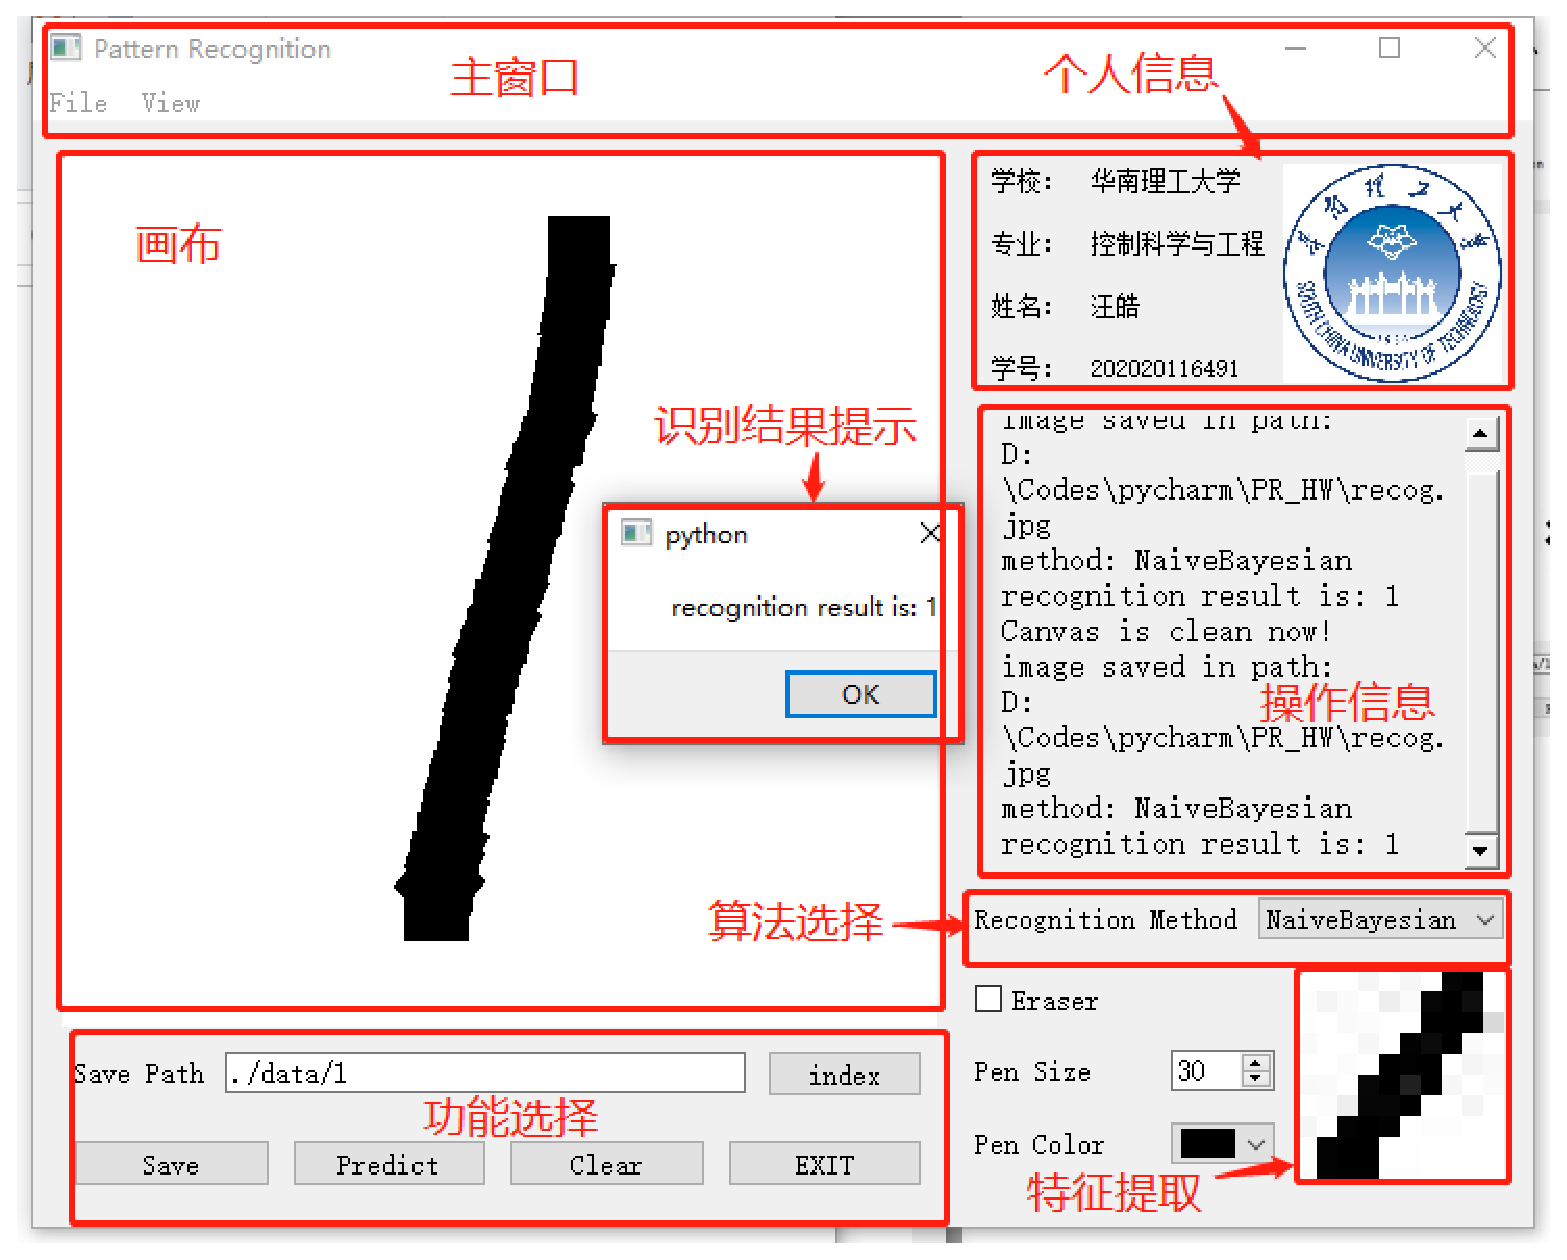
\includegraphics[scale=0.5]{./img/GUI.eps}
			\caption{GUI界面展示}
			\label{fig:2.2}
			\end{figure}	
\clearpage
\chapter{数据集}
	\section{手写数据集}
		利用GUI的画布手写数字,分为训练集和测试集,并按数字名存到文件夹中,文件目录如下所示。其中,训练集中每个数字有20张图片,测试集中每个数字有10张图片。
		\begin{figure}[!h]
			\centering
			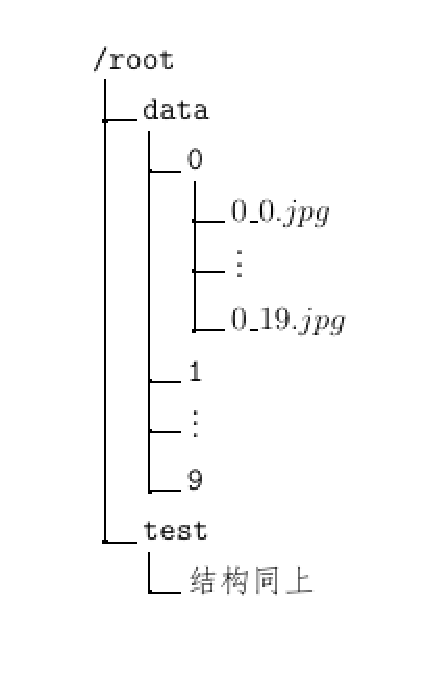
\includegraphics[scale=0.8]{./img/DataDirTree.eps}
			\caption{数据集文件目录}
			\label{fig:3.1}
		\end{figure}

	\section{MNIST数据集}
		对于CNN,其训练需要大数据的支持,故我们使用MNIST数据集。MNIST数据集由美国国家标准与技术研究所(National Institute of Standards and Technology (NIST))发起整理,一共统计了来自250个不同的人手写数字图片,其中50\%是高中生,50\%来自人口普查局的工作人员。是机器学习领域中非常经典的一个数据集,由60000个训练样本和10000个测试样本组成,每个样本都是一张28*28像素的灰度手写数字图片。

		MNIST数据集分为4个部分,如下表所示:
		\begin{table}[!h]
		\centering
		\caption{MNIST数据集简介}  
		\begin{tabular*}{9cm}{ll}  
		\hline  
		文件内容 & 文件用途 \\  
		\hline  
		\hline
		train-images-idx3-ubyte.gz  & 训练集图像 \\  
		train-labels-idx1-ubyte.gz  & 训练集标签 \\  
		t10k-images-idx3-ubyte.gz & 测试集图像\\
		t10k-labels-idx1-ubyte.gz & 测试集标签\\  
		\hline  
		\end{tabular*}  
		\end{table} 

	\section{特征处理}
		\subsection{目的}
			物理和结构上的特征通常易于为人的直觉感知,但有时难以定量描述,因而不易用于机器判别。而数学上的特征易于用机器定量描述和判别,故通常使用数学特征作为模式识别任务的特征描述,例如基于统计的特征。

			但对于一幅图像而言,例如我们的手写数字图像,尺寸是420*420,即使不考虑色彩,也至少有17万多个像素值作为原始特征。而每一个特征点的取值从0-255共有256个取值可能。原始这一幅图几十万的像素特征样本分布很稀疏,高维特征计算量大、冗余性高,且不能反映对象的本质。因而,特征处理的一个重要任务或目的就是从如此繁多的特征中选择其中的重要特征以减少特征数量,同时尽量保留分类信息。

		\subsection{处理方法}
			通常能够提取有效信息、压缩特征空间的特征处理方法有:特征提取和特征选择。所谓特征提取是用映射或变换的方法把原始特征变换为较少的新特征。而特征选择是指从原始特征中挑选出一些最有代表性、分类性能最好的特征。
		
			由于CNN算法的训练和测试是用MNIST手写数据集完成,故 我们希望最后的特征与MNIST数据集类似,即满足以下条件:
			\begin{enumerate}[itemindent=1em]
				\renewcommand{\labelenumi}{\theenumi)}
				\item 每个特征之间尽量独立分布;
				\item 特征图用的灰度图表示;
				\item 特征大小为28*28;
				\item 特征图尽量在中央,且用黑底白字表示。
			\end{enumerate}

			于是,我们将图像有效范围从420*420的像素阵中分割出来,放回到原图中央并缩小到28*28,再转换成灰度图,翻转后得到一个尺寸为28*28维的特征图,其中间过程如图3.2所示。
			\begin{figure}[!h]
			\centering
			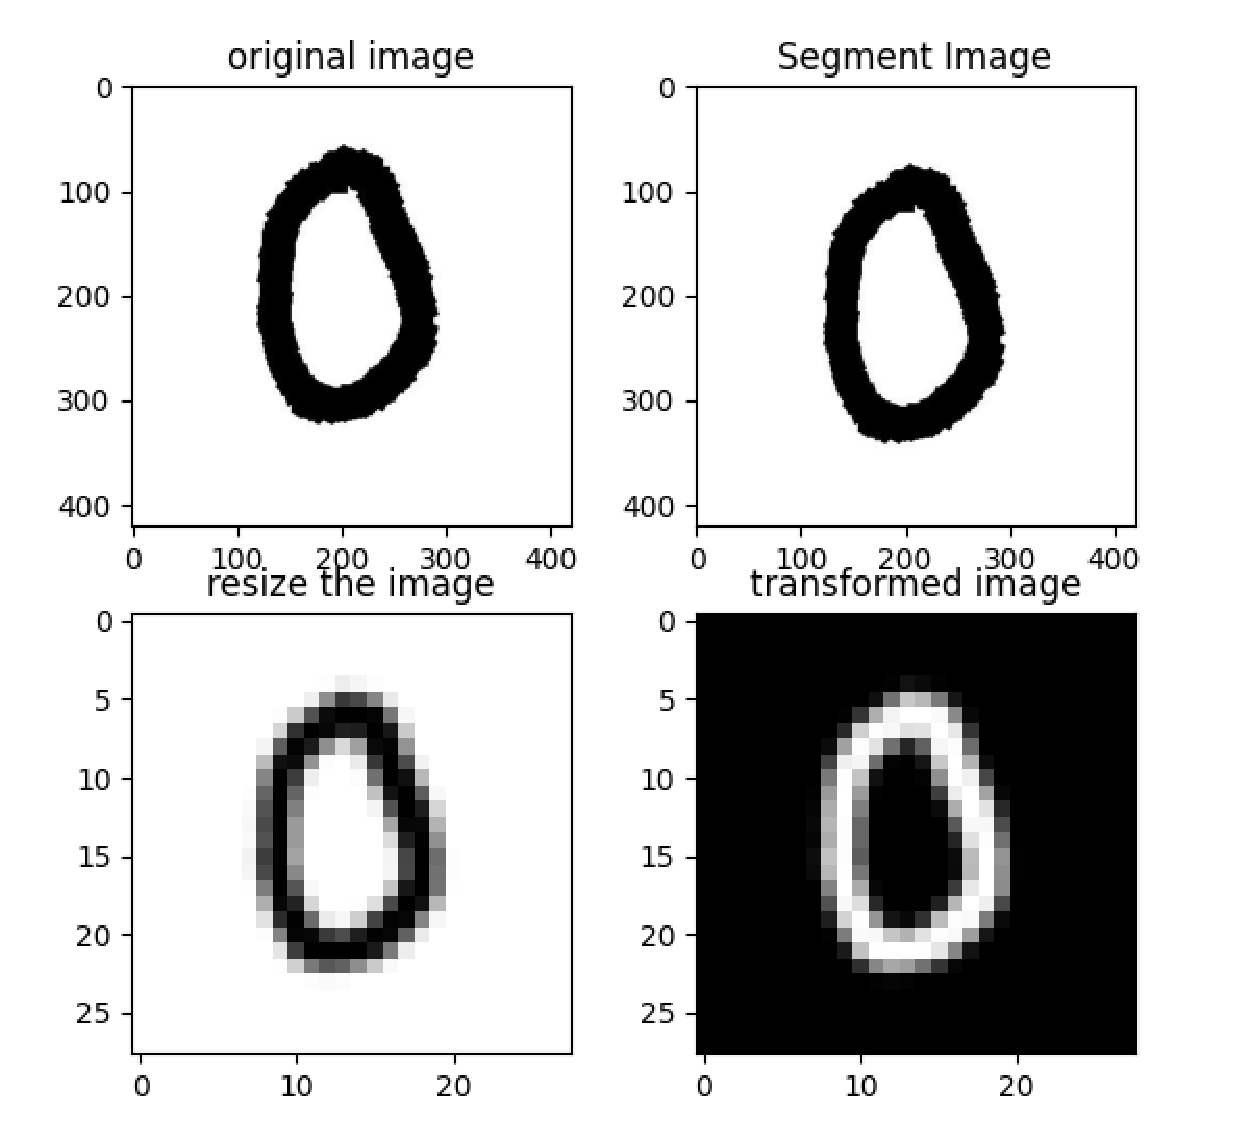
\includegraphics[scale=0.5]{./img/FeatureMapping.eps}
			\caption{特征处理过程}
			\label{fig:3.2}
			\end{figure}
\clearpage

\chapter{卷积神经网络}
	\section{CNN介绍}
		卷积神经网络(Convolutional Neural Networks, CNN)是一类包含卷积计算且具有深度结构的前馈神经网络(Feedforward Neural Networks),是深度学习(deep learning)的代表算法之一。卷积神经网络具有表征学习(representation learning)能力,能够按其阶层结构对输入信息进行平移不变分类(shift-invariant classification),因此也被称为“平移不变人工神经网络(Shift-Invariant Artificial Neural Networks, SIANN)。

		对卷积神经网络的研究始于二十世纪80至90年代,时间延迟网络和LeNet-5是最早出现的卷积神经网络 。伴随着多层感知器、SVM等分类器,CNN网络经过三起三落,终于在2010年前后,随着深度学习理论的提出和数值计算设备的改进,以及大数据和GPU等技术的发展,卷积神经网络得到了快速发展,并被应用于计算机视觉、自然语言处理等领域。

		卷积神经网络仿造生物的视知觉(visual perception)机制构建,可以进行监督学习和非监督学习,其隐含层内的卷积核参数共享和层间连接的稀疏性使得卷积神经网络能够以较小的计算量对格点化(grid-like topology)特征,例如像素和音频进行学习、有稳定的效果且对数据没有额外的特征工程(feature engineering)要求。

	\section{结构}
		\subsection{输入层}
		卷积神经网络的输入层可以处理多维数据,常见地,一维卷积神经网络的输入层接收一维或二维数组,其中一维数组通常为时间或频谱采样;二维数组可能包含多个通道;二维卷积神经网络的输入层接收二维或三维数组;三维卷积神经网络的输入层接收四维数组。

		该层要做的处理主要是对原始图像数据进行预处理,其中包括:
		\begin{enumerate}[itemindent=1em]
			\renewcommand{\labelenumi}{\theenumi)}
			\item 去均值:把输入数据各个维度都中心化为0,如图4.1所示,其目的就是把样本的中心拉回到坐标系原点上;
			\item 归一化:幅度归一化到同样的范围,如图4.1所示,即减少各维度数据取值范围的差异而带来的干扰,比如,我们有两个维度的特征A和B,A范围是0到10,而B范围是0到10000,如果直接使用这两个特征是有问题的,好的做法就是归一化,即A和B的数据都变为0到1的范围;
			\item PCA:用PCA降维;
			\item 白化:白化是对数据各个特征轴上的幅度归一化。
		\end{enumerate}
		\begin{figure}[!h]
		\centering
		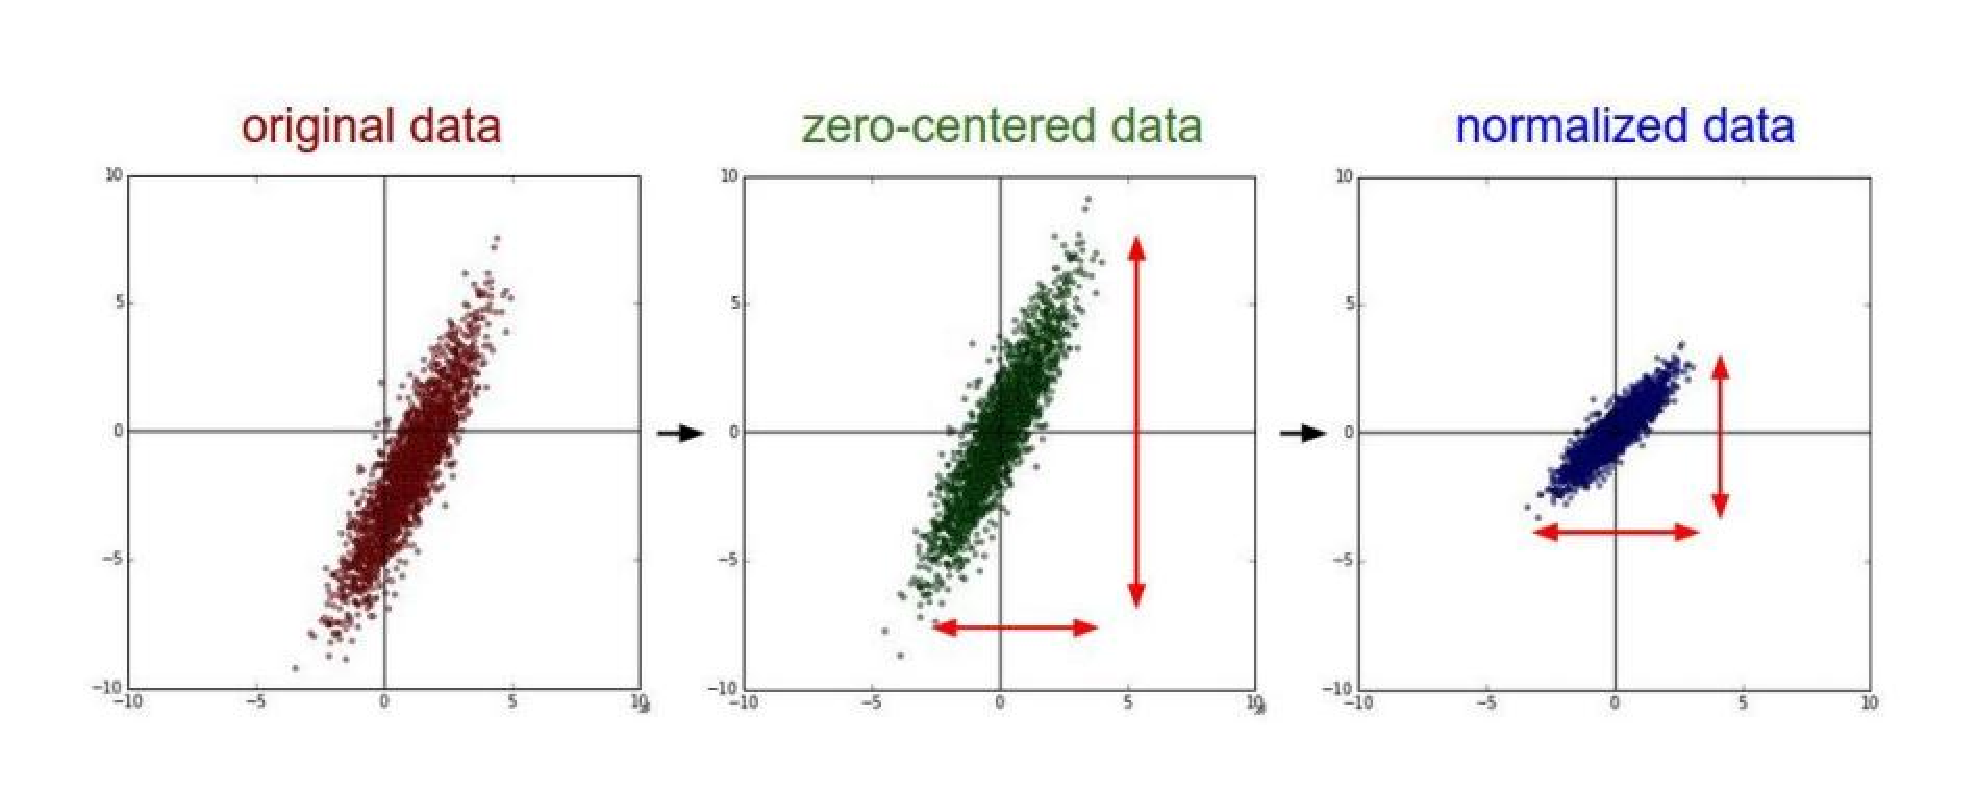
\includegraphics[scale=0.45]{./img/Norm.eps}
		\caption{去均值及归一化}
		\label{fig:4.1}
		\end{figure}

		\subsection{卷积层}
			这一层就是卷积神经网络最重要的一个层次,也是“卷积神经网络”的名字来源。
	
			在这个卷积层,有两个关键操作:
			\begin{enumerate}[itemindent=1em]
				\renewcommand{\labelenumi}{\theenumi)}
				\item 局部关联。每个神经元看做一个滤波器(filter);
				\item 窗口(receptive field)滑动, filter对局部数据计算。
			\end{enumerate}
	
			卷积层有如下几个名词:
			\begin{enumerate}[itemindent=1em]
				\renewcommand{\labelenumi}{\theenumi)}
				\item 深度/depth:如图4.2;
				\item 步长/stride:窗口一次滑动的长度;
				\item 填充值/zero-padding:为了保证每次窗口滑动之后,图像大小不会变所设置的填充图片像素值。
			\end{enumerate}
			\begin{figure}[!h]
			\centering
			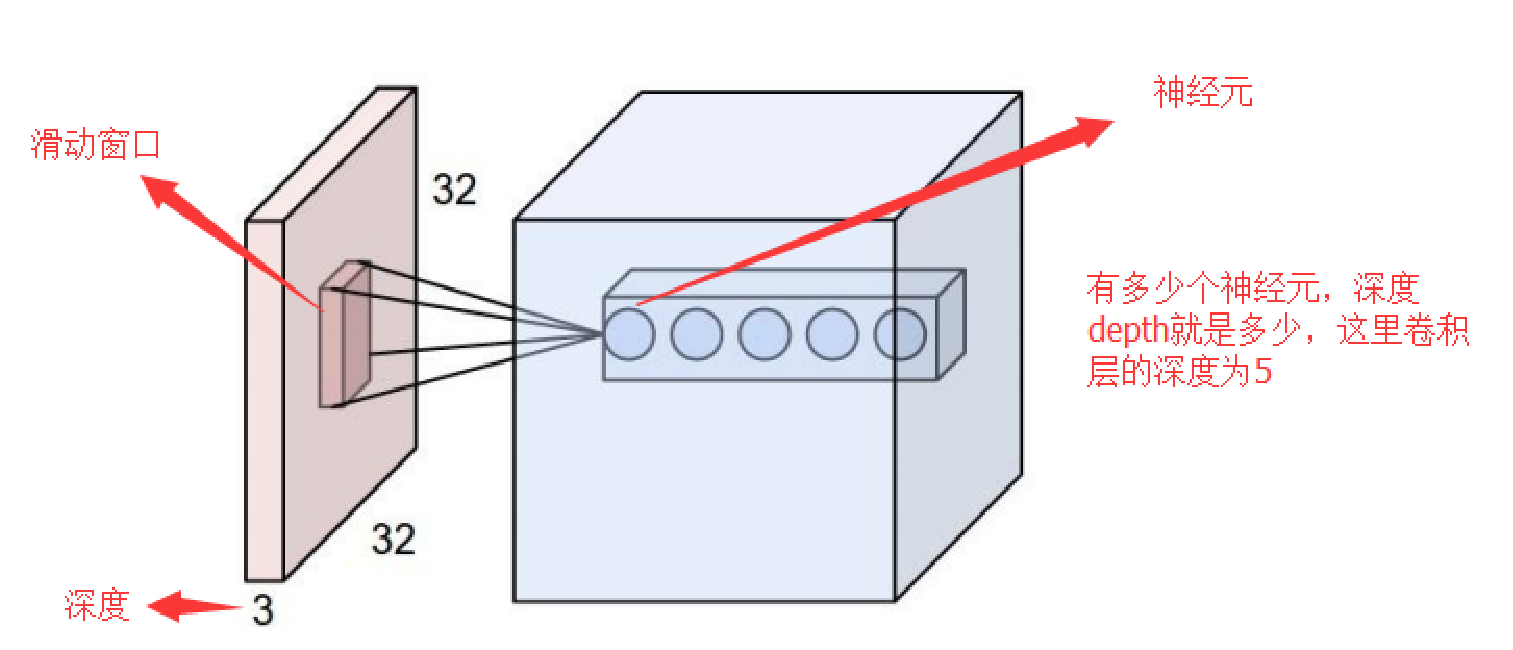
\includegraphics[scale=0.45]{./img/Depth.eps}
			\caption{卷积神经网络的深度概念}
			\label{fig:4.2}
			\end{figure}
	
			同时,为了减少参数,卷积神经网络采用了参数共享机制。于是一次卷积运算即可由图4.3所示。
			\begin{figure}[!h]
			\centering
			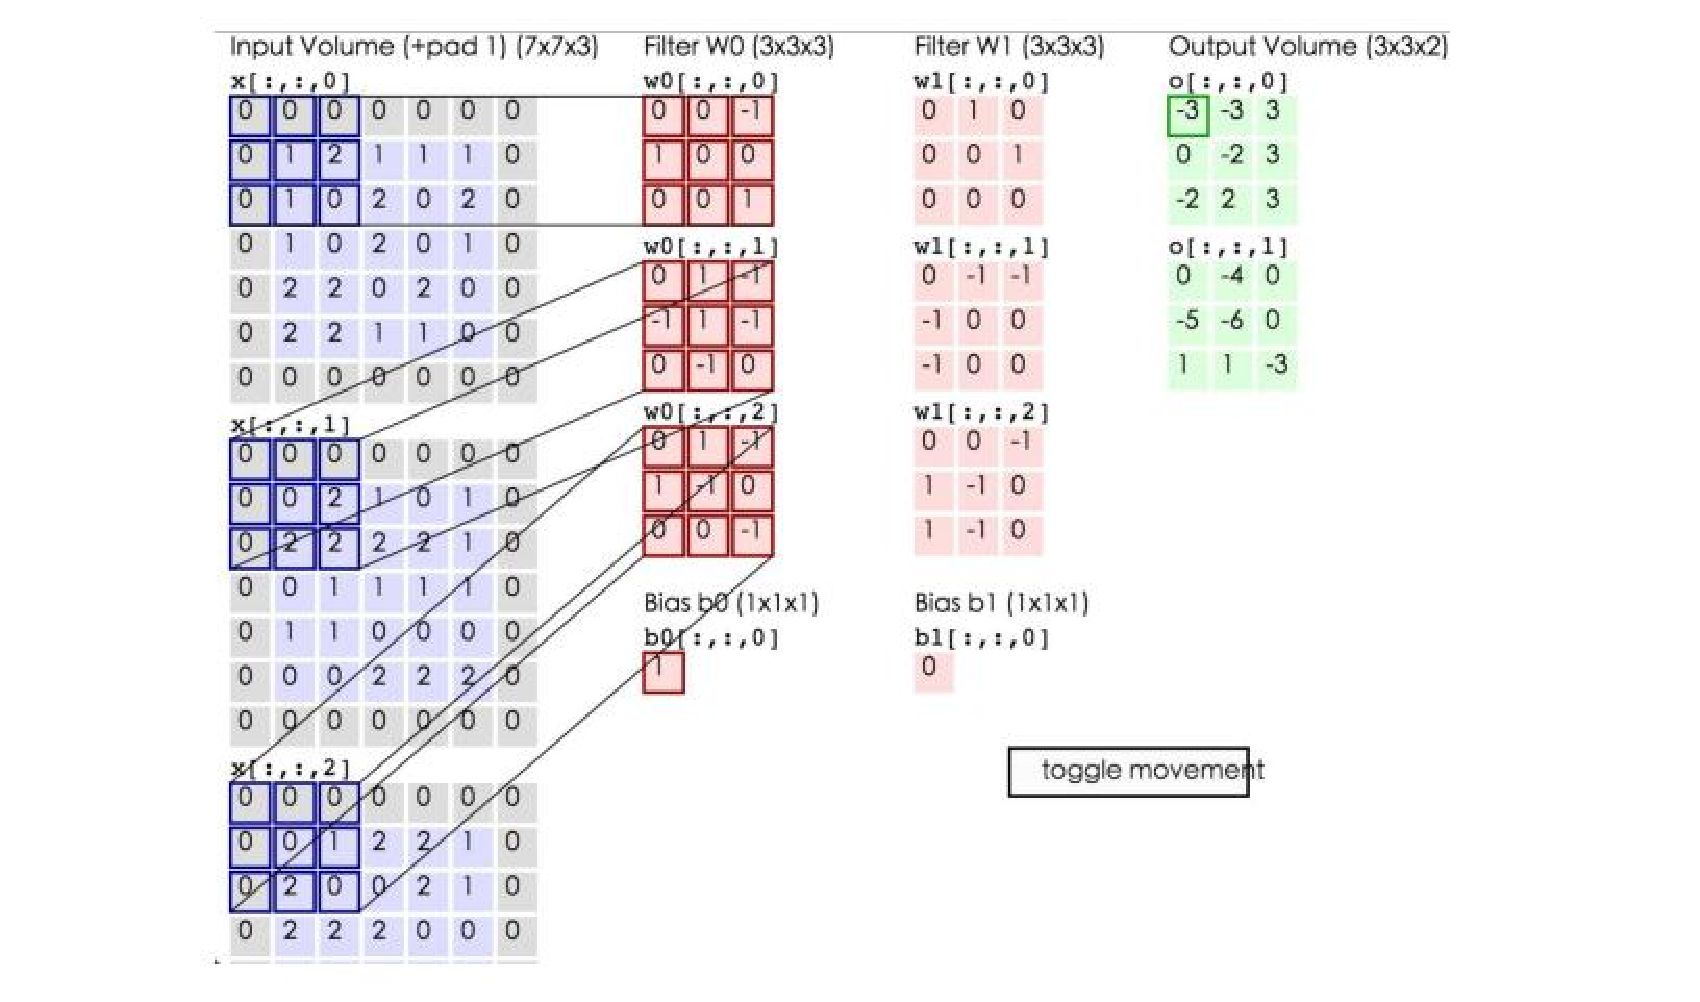
\includegraphics[scale=0.5]{./img/Kernel.eps}
			\caption{卷积计算示例}
			\label{fig:4.3}
			\end{figure}

		\subsection{激励层}
			如图4.4所示,激励层的作用是把卷积层输出结果做非线性映射。
			\begin{figure}[!h]
			\centering
			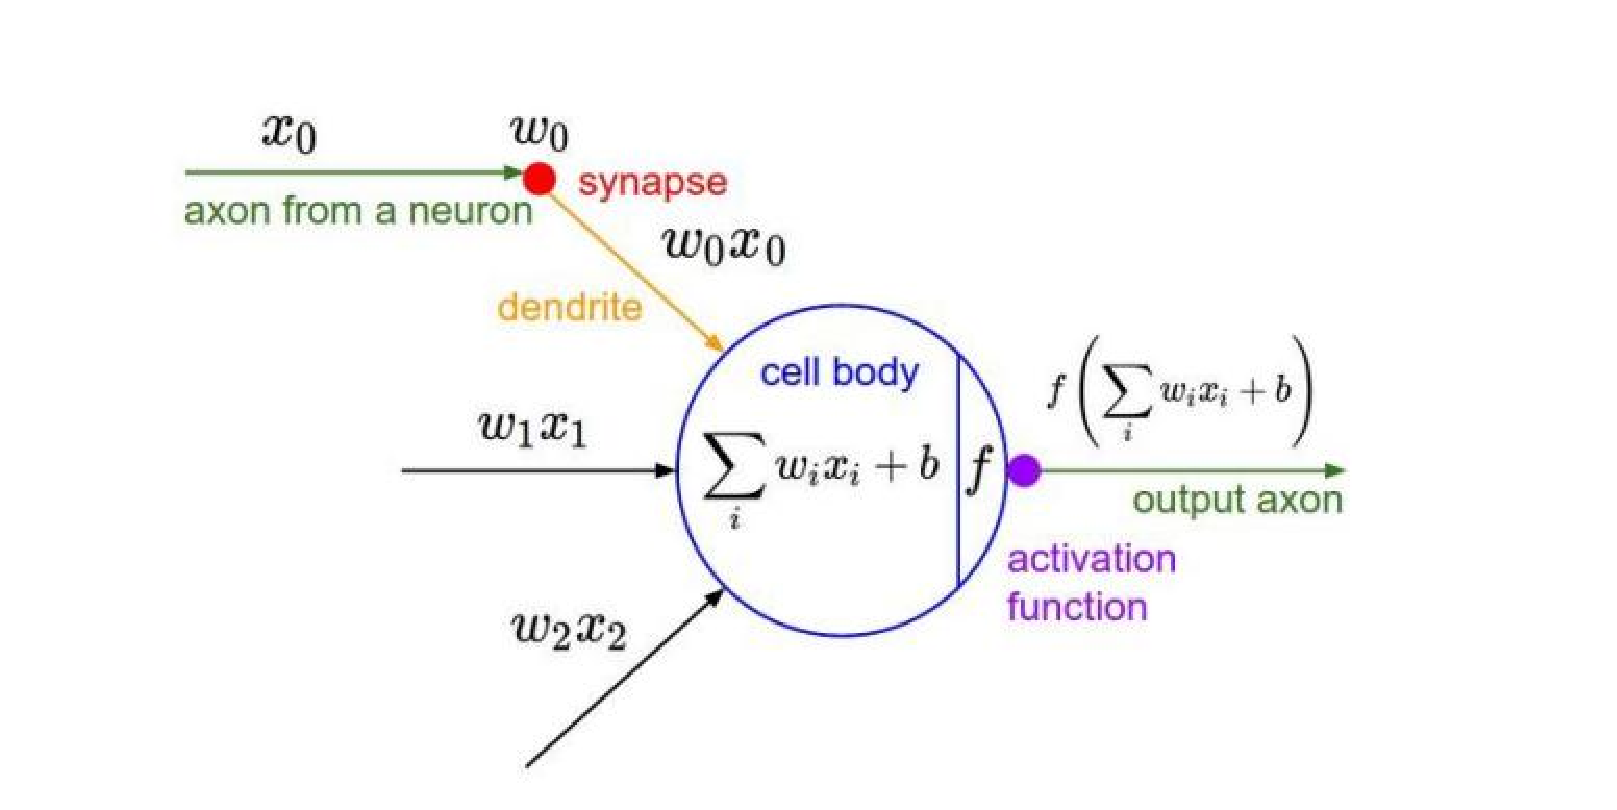
\includegraphics[scale=0.4]{./img/Active.eps}
			\caption{激励函数示意图}
			\label{fig:4.4}
			\end{figure}

			CNN采用的激励函数一般为ReLU(The Rectified Linear Unit/修正线性单元),它的特点是收敛快,求梯度简单,但较脆弱,图像如图4.5所示,公式如式4.1。
			\begin{figure}[!h]
			\centering
			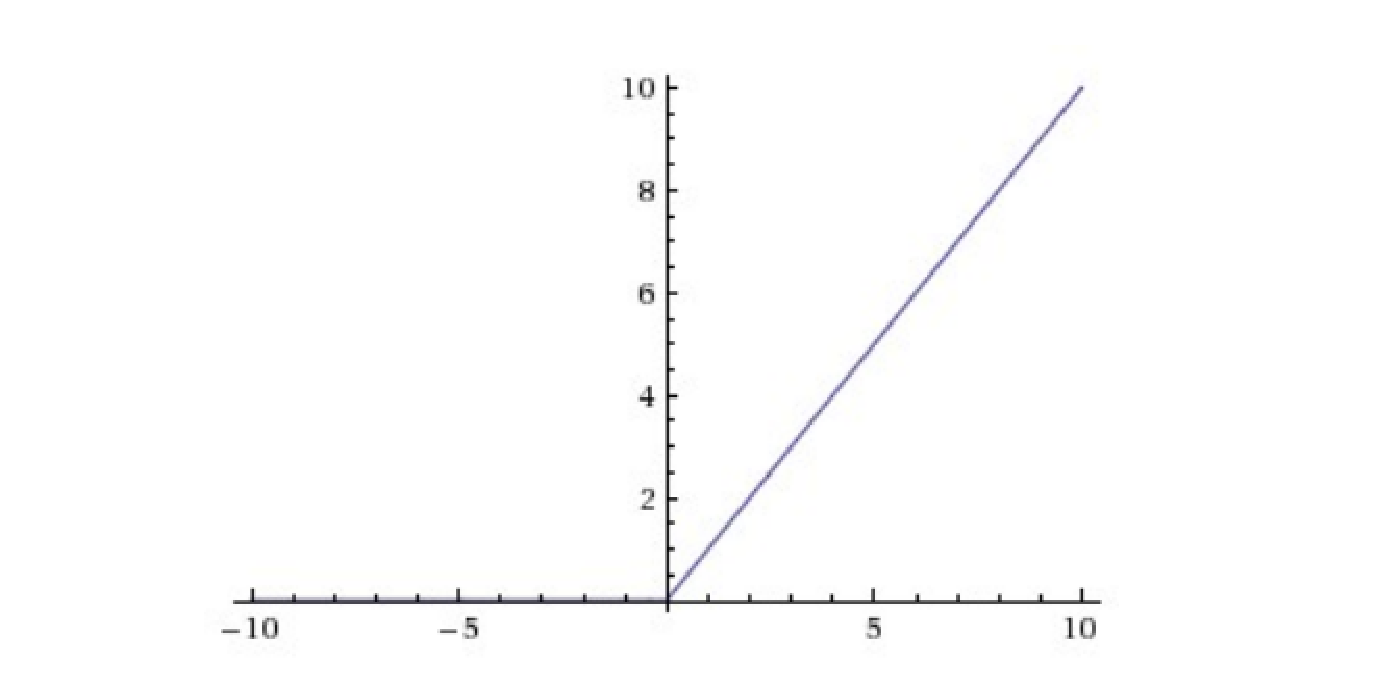
\includegraphics[scale=0.5]{./img/ReLU.eps}
			\caption{激活函数ReLU图像}
			\label{fig:4.5}
			\end{figure}
			\begin{equation}
			ReLU(\bm{x})=\left\{
			\begin{array}{rcl}
			\bm{x} & & {\bm{x} \geq 0}\\
			0 & & {\bm{x}<0}
			\end{array} \right.
			\end{equation}

		\subsection{池化层}
			池化层夹在连续的卷积层中间, 用于压缩数据和参数的量,减小过拟合,如图4.6所示。
			\begin{figure}[!h]
			\centering
			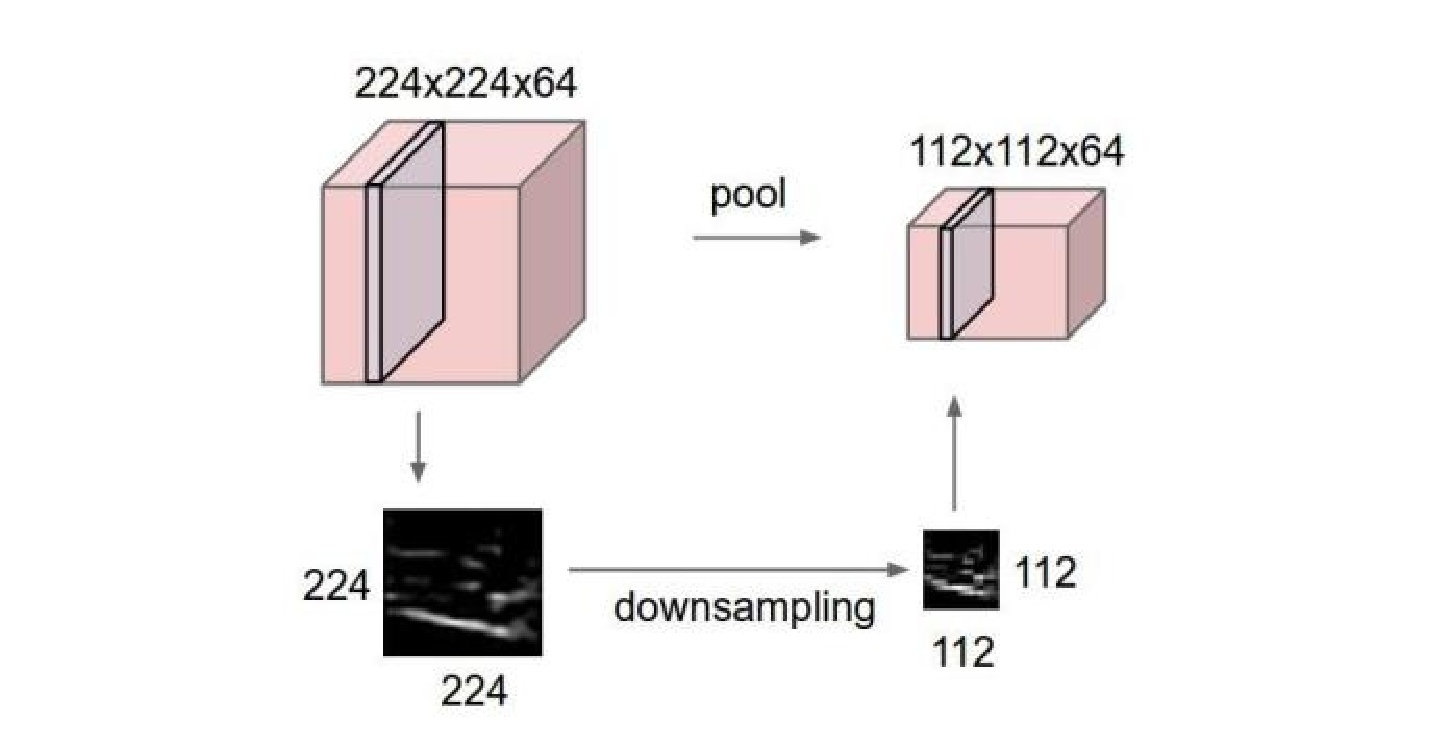
\includegraphics[scale=0.5]{./img/Pooling.eps}
			\caption{MaxPooling的机理}
			\label{fig:4.6}
			\end{figure}

			池化层的具体作用如下:
			\begin{enumerate}[itemindent=1em]
				\renewcommand{\labelenumi}{\theenumi)}
				\item 特征不变性:也就是特征的尺度不变性,池化操作就是图像的resize,图像压缩时去掉的信息只是一些无关紧要的信息,而留下的信息则是具有尺度不变性的特征,是最能表达图像的特征;
				\item 特征降维:把冗余信息去除,把最重要的特征抽取出来;
				\item 在一定程度上防止过拟合,更方便优化。
			\end{enumerate}

		\subsection{全连接层}
			即机器学习常见的分类器。由于我们采用梯度下降算法来更新参数,故一般全连接层使用多层感知器。

	\section{CNN设计}
		设计一个浅层的CNN网络,如图4.7所示。
		\begin{figure}[!h]
		\centering
		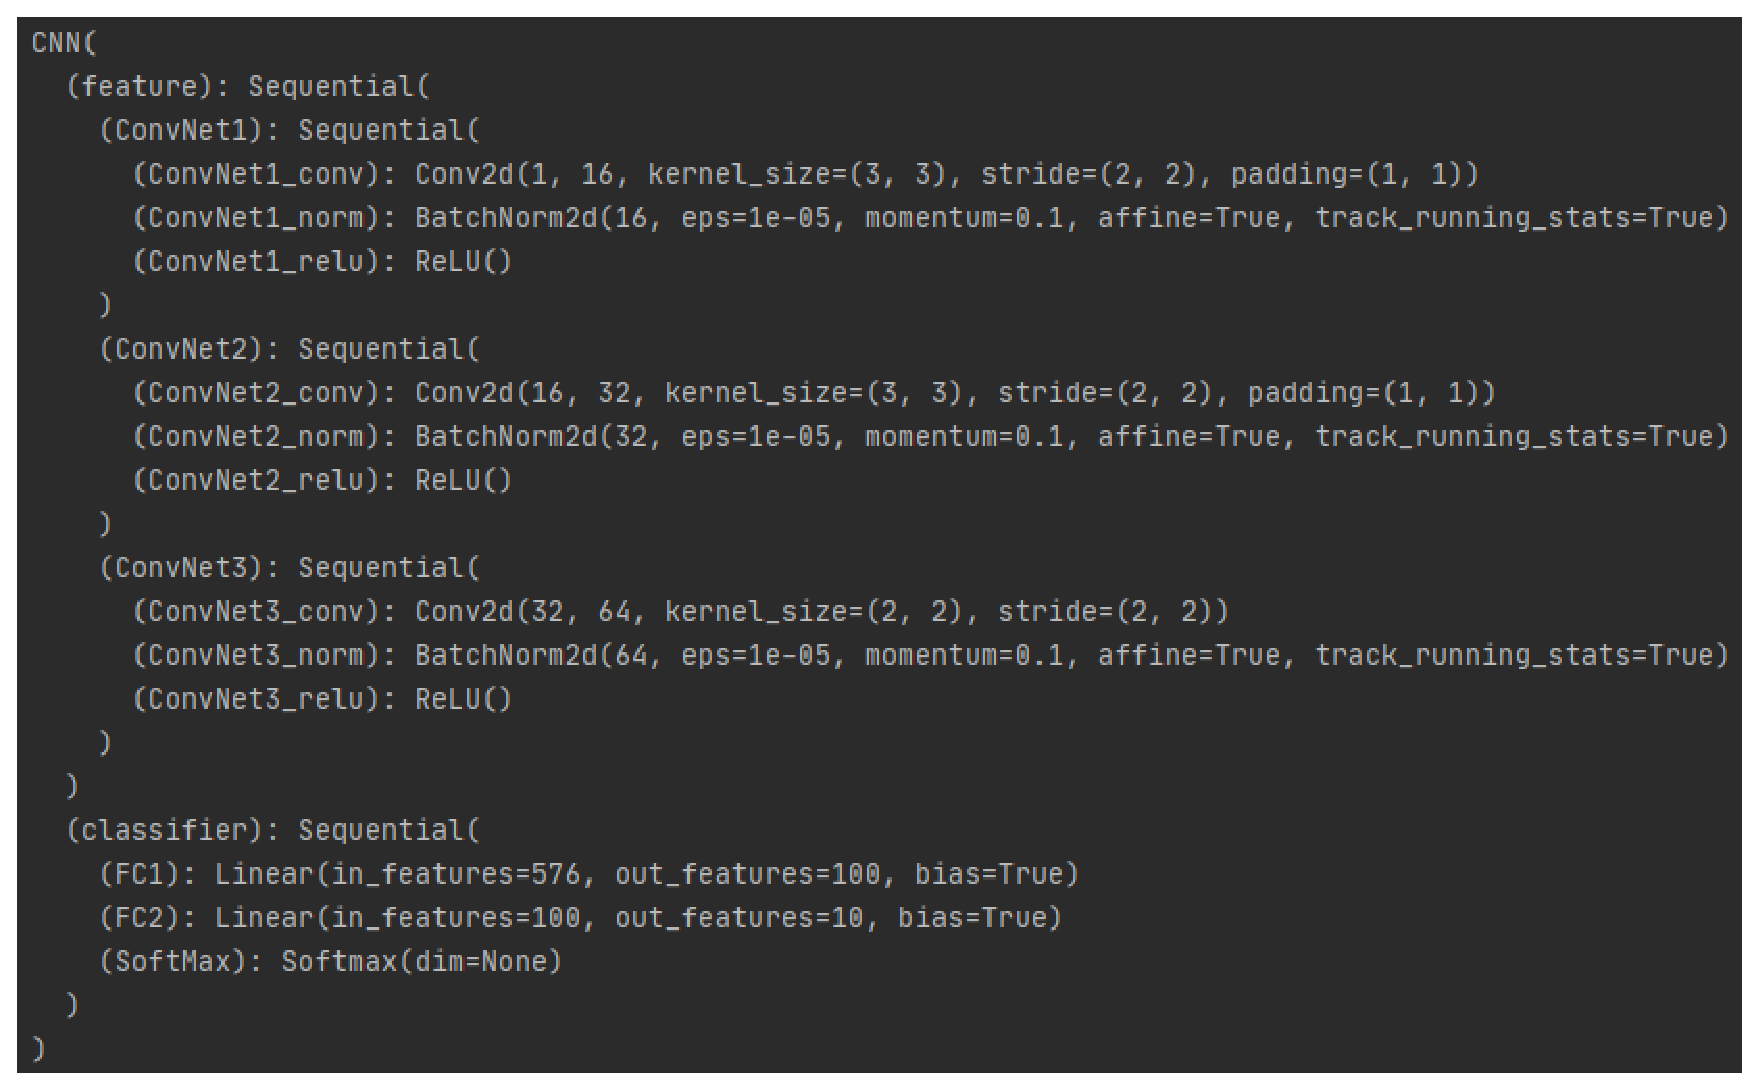
\includegraphics[scale=0.5]{./img/CNNPrint.eps}
		\caption{CNN网络结构}
		\label{fig:4.7}
		\end{figure}

	\section{CNN实现}
		使用 $pytorch$ 库实现如图4.7中CNN网络,并在 $tensorboard$ 中进行可视化,得到图4.8。

		使用MNIST数据集对网络进行训练和测试。训练时,使用50000张训练集,同时用2000张测试集作为验证以选取最好的模型。设置超参数训练次数 $epoch=200$、学习率为$lr=0.001$、正则项$wc=1e-4$、单次训练量$batch=256$。反向传播算法采用Adam(Adaptive Moment Estimation)(其本质上是带有动量项的RMSprop,利用梯度的一阶矩估计和二阶矩估计动态调整每个参数的学习率。它的优点主要在于经过偏置校正后,每一次迭代学习率都有个确定范围,使得参数比较平稳)。损失函数为交叉熵函数,训练完成后,存储最后训练的模型和在验证集上表现最好的模型。对于后者,得到训练集准确率为99.8\%,测试集准确率为98.82\%。
		\begin{figure}[!h]
		\centering
		\subfigure[CNN的整体模块]{
		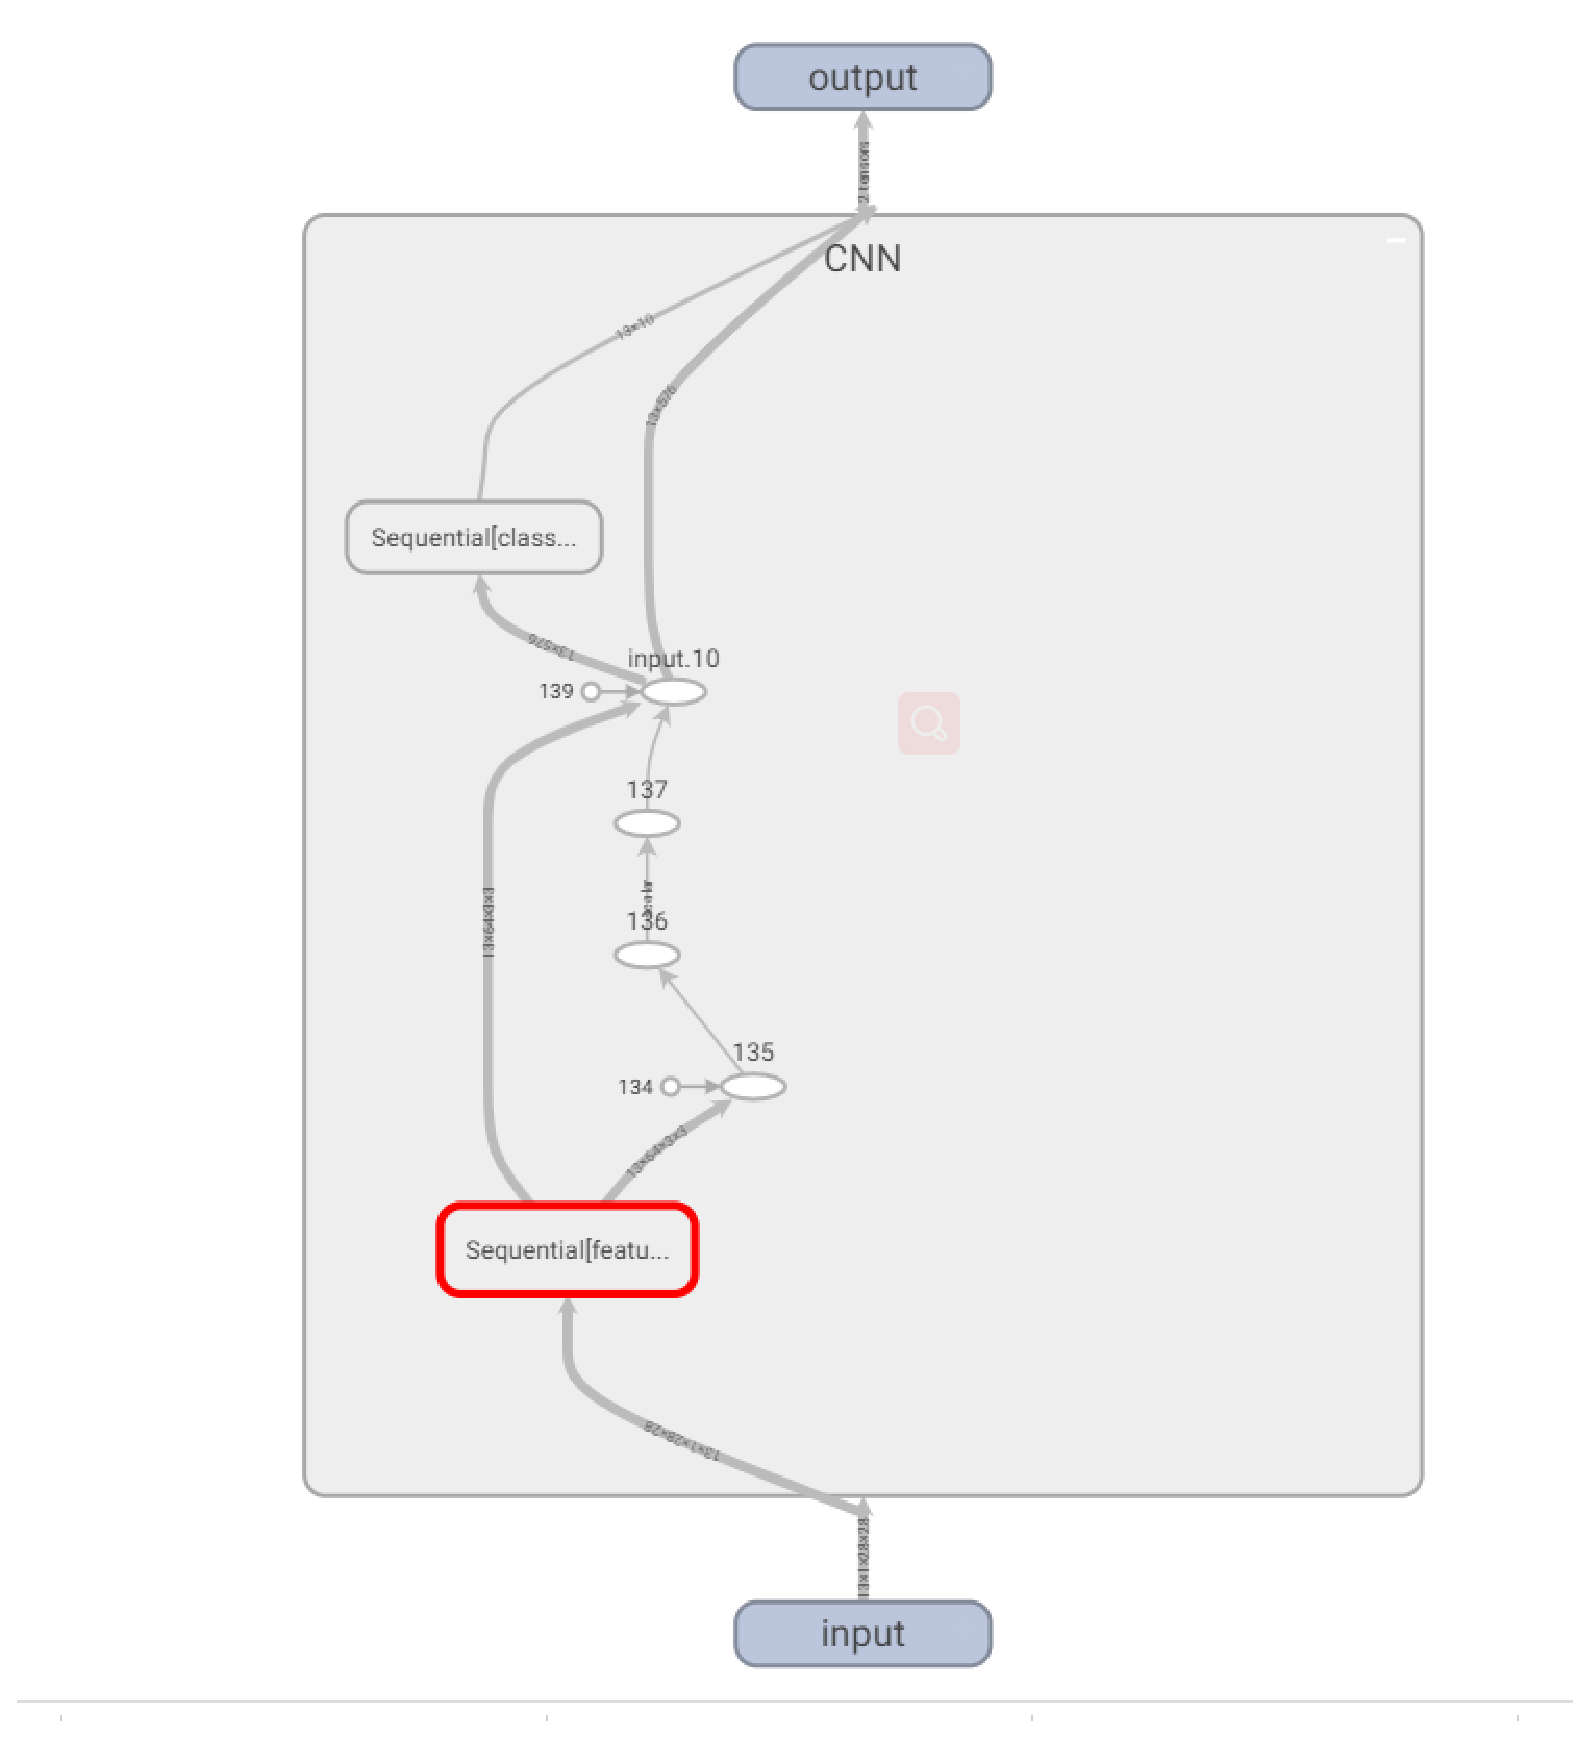
\includegraphics[height=5cm]{./img/CNNImage.eps}
		}
		\quad
		\subfigure[CNN单层卷积层]{
		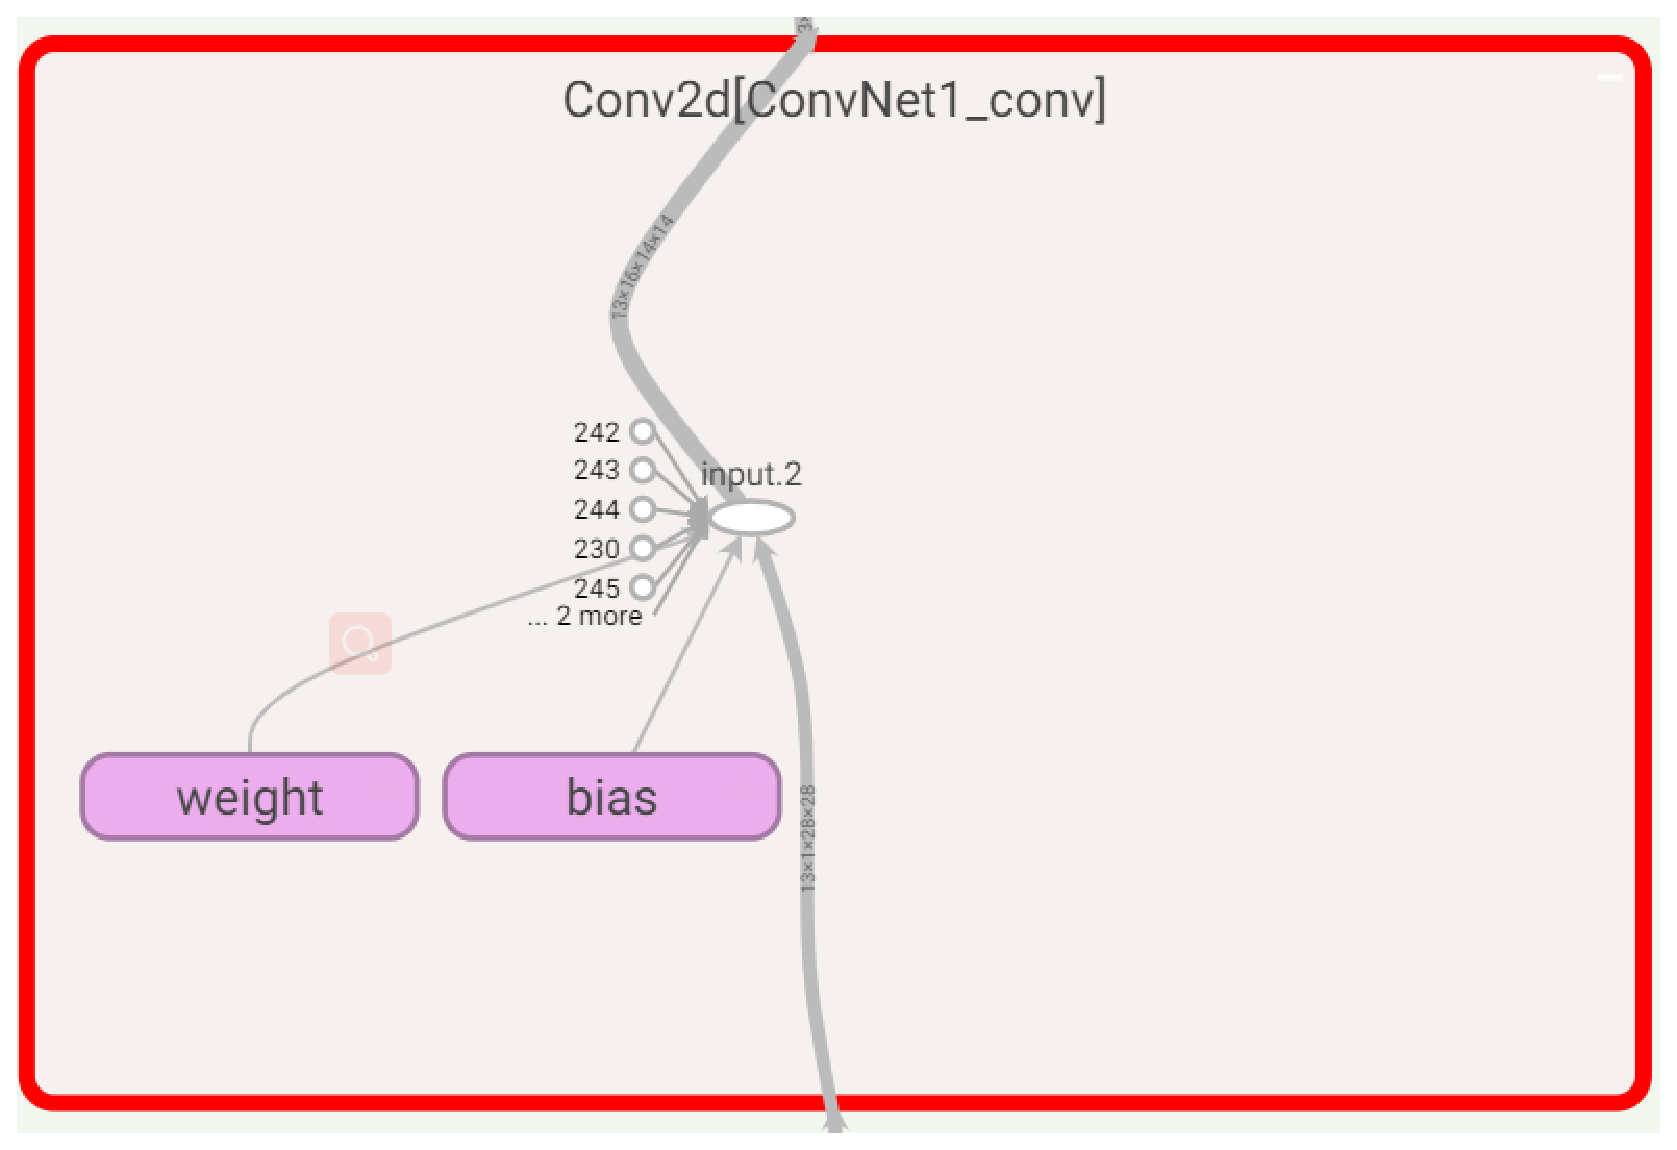
\includegraphics[height=5cm]{./img/InLayer.eps}
		}
		\quad
		\subfigure[CNN的特征提取模块展开]{
		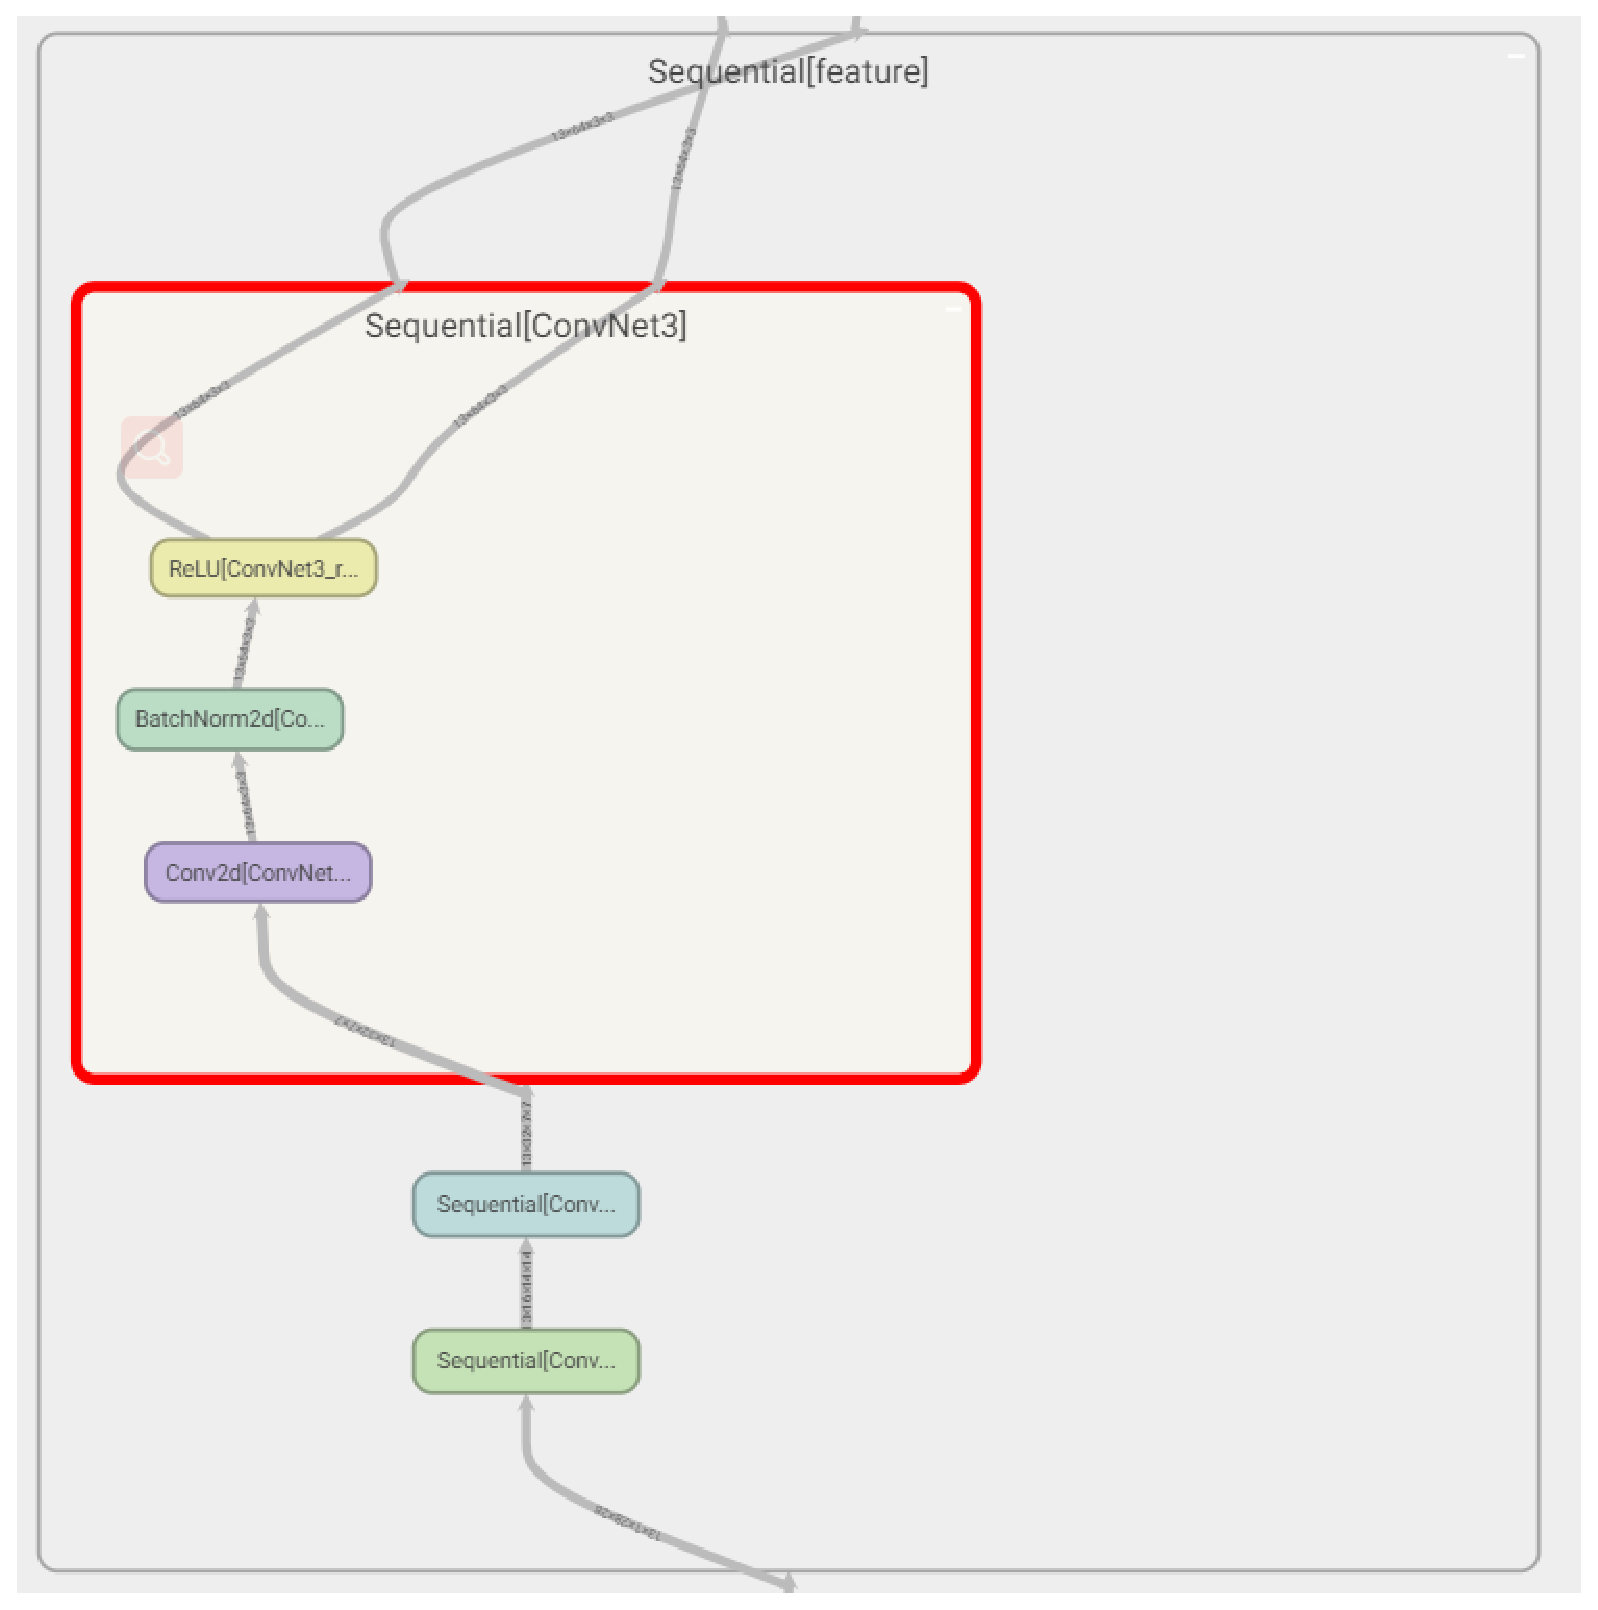
\includegraphics[height=5cm]{./img/FeatureLayer.eps}
		}
		\quad
		\subfigure[CNN的线性分类模块展开]{
		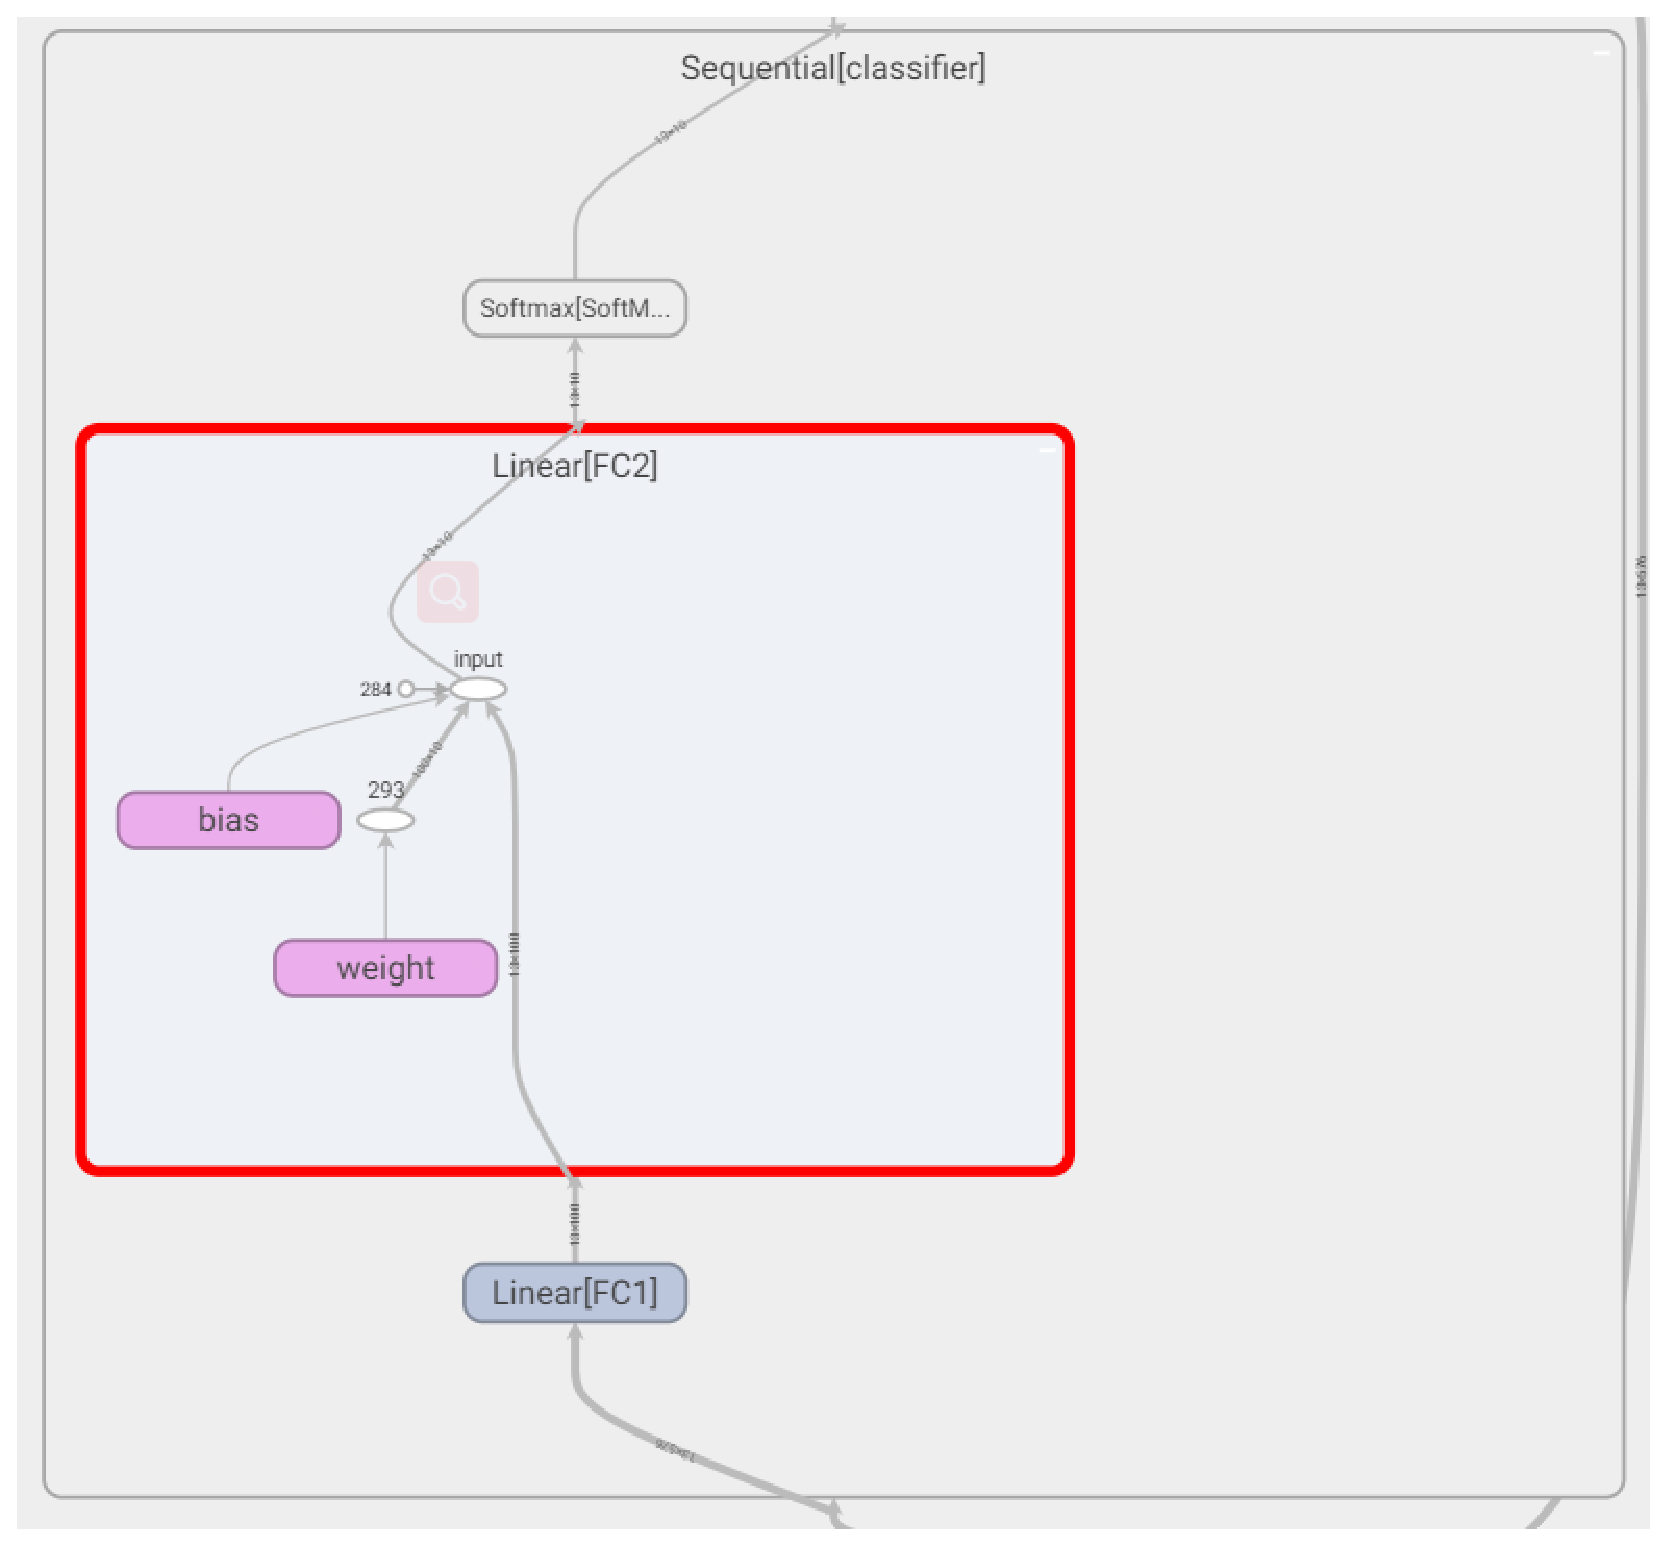
\includegraphics[height=5cm]{./img/Dense.eps}
		}
		\quad
		\subfigure[Acc和Loss]{
		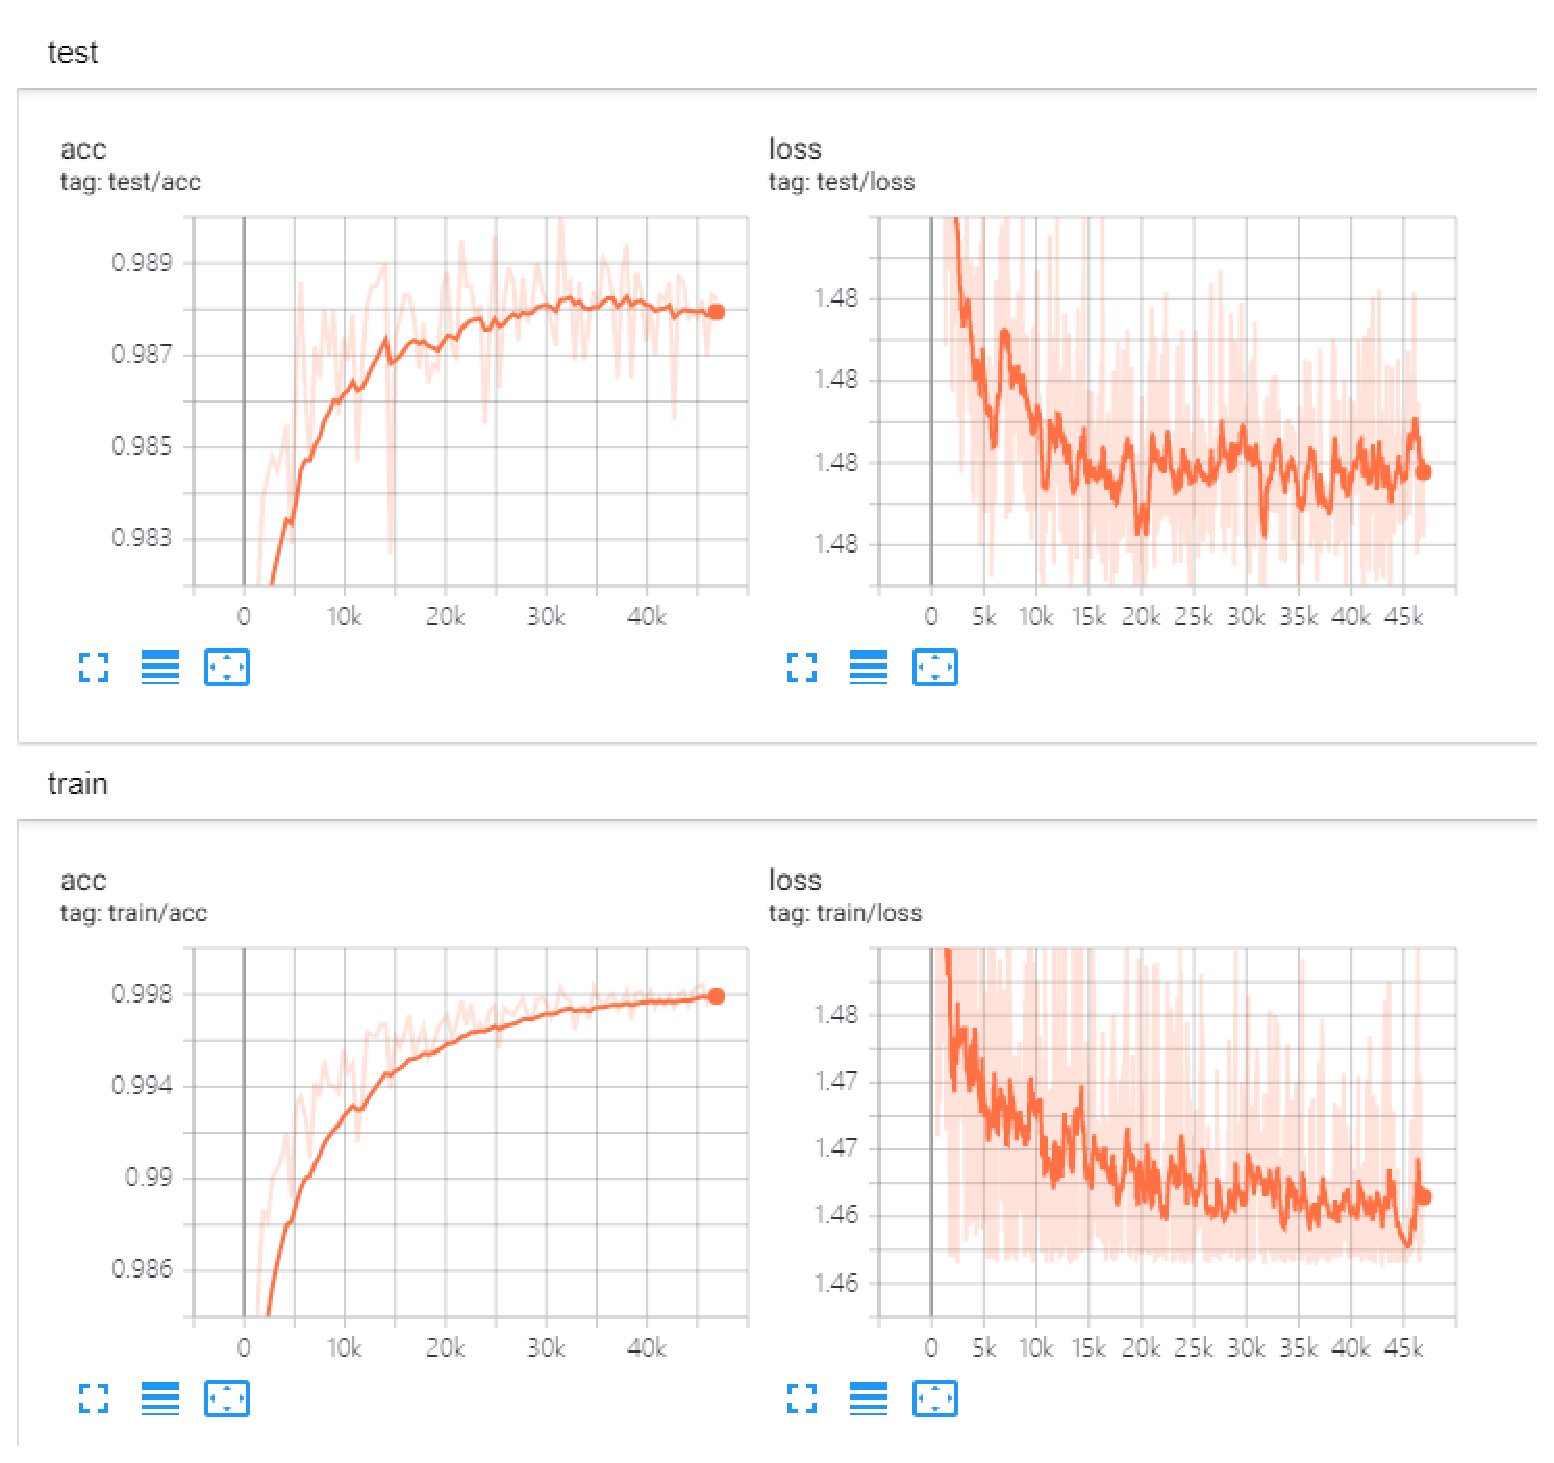
\includegraphics[height=5cm]{./img/Loss.eps}
		}
		\quad
		\subfigure[数字0特征提取层输出]{
		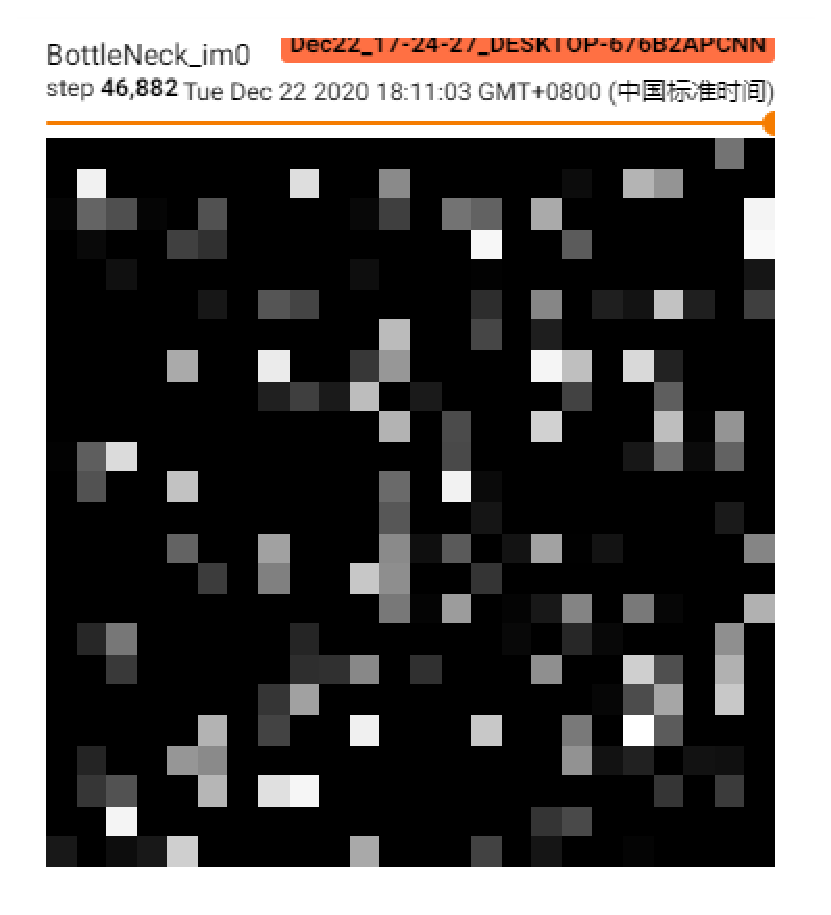
\includegraphics[height=5cm]{./img/BottleNeck.eps}
		}
		\caption{tensorboard可视化CNN}
		\end{figure}

		将我们自己的数据集经过特征提取后进行测试,得到准确率为88\%。如上图f)所示,对特征提取层做可视化提取可以发现,CNN网络对图像经过一系列运算后提取到了一些特征,用于计算。
\clearpage
\end{document}